\section{Results}
\subsection*{\textbf{1a):} Local energy}
The local energy is  derived and presented in appendix \ref{app:el}


\subsection*{\textbf{1b):} Developing your code and \textbf{1d):} A better statistical analysis}

The results of the simulations are included in the appendix \ref{app:fig}as figures \ref{fig:1b_1} \ref{fig:1b_10}, \ref{fig:1b_100} and \ref{fig:1b_500}. The results were produced with the file \lstinline{main_b.cpp}\footnote{at commit \lstinline{b0ff612bc6666335b106af5e22a7a13a13c7cff7}}. Errors in the expectation value for the energy in the plots are computed with the blocking method\footnote{the blocking implementation is a copy of the code in Ref. \cite{ComphysGit}}. The errors are presented as errorbars in the plots referenced above.
The exact answer for the minimum of the expecation value of the energy can be derived from equation \ref{eq:el_ni}. The minimum of the local energy has to be where the kinetic and potential energies cancel exactly. In the case of the 3d particle we see the following after imposing units in terms of the characteristic lengths and frequencies of the harmonic oscillator. 

\begin{align}
\mathfrak{min}(E_L)  \implies \left(\frac{1}{2}\right)[4\alpha^2 (x^2 + y^2 + \beta^2 z^2) ] &= \frac{1}{2} (x^2 + y^2 + \beta z^2) \\
 2 \alpha ^2  &= \frac{1}{2} \\
 \alpha &= 0.5
\end{align}
With $\alpha$ at the minimum we then expect the following values for $\expect{E}$
\begin{equation}
\begin{split}
\text{1D: }E_L |_{\alpha = 0.5} &= \sum_i^N \alpha = N \alpha,\\
\text{2D: }E_L|_{\alpha = 0.5} &= \sum_i^N  2\alpha = 2N \alpha \\
\text{3D: }E_L|_{\alpha = 0.5} &= \sum_i^N  2\alpha + \alpha \beta  = 3N\alpha
\end{split}
\end{equation}
In general the energy in the non-interactive case at the variational minimum for our trial wavefunction can then be expressed as 
\begin{equation}
\mathfrak{min}(\expect{E[\alpha]}) = 0.5 \cdot N \cdot D  
\end{equation}
Where $N$ is the number of particles and $D$ is their dimension. From the figures referenced in the beginning of this section it is clear that both the numerical and analytic solutions have a minimum at that  agrees with the analytical solution. The intervals  were chosen such that the known optimum for $\alpha$ was included, this information in in general not available and motivated the gradient descent algorithm implemented for task 1.f. From the figures referenced above it is also noted that there is a substantial time difference in the numeric and analytic algorithms. 

\subsection*{\textbf{1e:} The repulsive interaction}


In Table \ref{tab:Re.int.} we see the results for the case of the elliptical trap with a repulsive interaction. We have used the Hamiltonian in Equation \ref{eq:elliptical} to solve this case. The analytic solution of the local energy can be found in Appendix 1. The code that was used to find these results can be found \lstinline{gaussian_inter_analytic.cpp}\footnote{at commit \lstinline{d1c9ec9cc5640e7030b18adbabc802d2414dba75}}.
We have used $a = 0.0043$ and $\beta = 2.82843$. We see that the expectation value of the local energy increases slowly as we increase the number of particles. It can seem that this is the case of the variational parameter $\alpha$ as well. 
As for the CPU-time it increases rapidly. Already for 100 particles we are closing in one 3 hours.


\begin{table}[]
    \centering
    \begin{tabular}{|c|c|c|c|c|c|}
    \hline
         $N$ & $\alpha$ & $\sigma^2$ & $\langle E_L \rangle$ & $\frac{\langle E_L \rangle}{N}$ & CPU-time [sek] \\
         \hline
         10 & 0.480013 & 1.73405e-06 & 21.643 & 2.1643 & 12.31 \\
         \hline
         50 & 0.480127 & 1.75833e-06 & 111.066 & 2.2213 & 1253.91\\
         \hline
         100 & 0.480279 & 1.75902e-06 & 228.682 & 2.2868 & 9854.01 \\
         \hline
    \end{tabular}
    \caption{VMC with Metropolis sampling. Calculations done in 3 dimensions with number of cycles $N_{MC} = 10^{6}$ for an elliptical trap, $\beta = 2.82843$ with interaction, $a = 0.0043$. Step length $t = 0.5$.}
    \label{tab:Re.int.}
\end{table}


\subsection*{\textbf{1f:} Finding the best parameter}
Applying the gradient descent algorithm to tune the variational parameter resulted in satisfying convergence to the optimal value for the variational parameter $\alpha$. The simulation results are included in figure \ref{fig:gd_nm_nia}\footnote{The simulations were produced with the file \lstinline{mainf_f.cpp} at commit \lstinline{2d03030ec5a711383d582dde23869483d122c6b6}}. After the convergence was shown to be satisfactory for the non-interactive case simulations were run for the hamiltonian with interaction \footnote{commit \lstinline{f285327a7d95349a874aafe16d8ecd5f48c5cef5}}. The resulting minimum for the variational parameter is slightly lower than for the non-interactive case with a value of $\alpha_{min} \approx 0.49888\ldots$. These findings are illustrated in figure \ref{fig:gd_nm_ia}. 


\begin{figure}
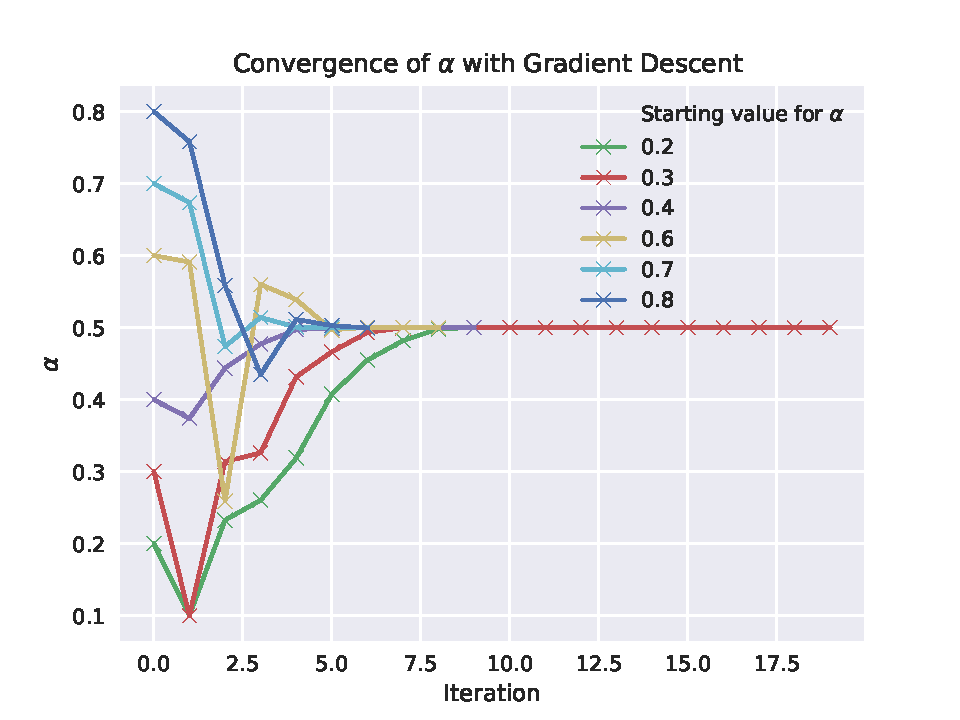
\includegraphics{figures/GD_NM_NIA.pdf}
\caption{Finding the optimal $\alpha$ with GD. This plot show the number of iterations it took to reach the minimum for the non-interactive spherical trap.}\label{fig:gd_nm_nia}
\end{figure} 

\begin{figure}
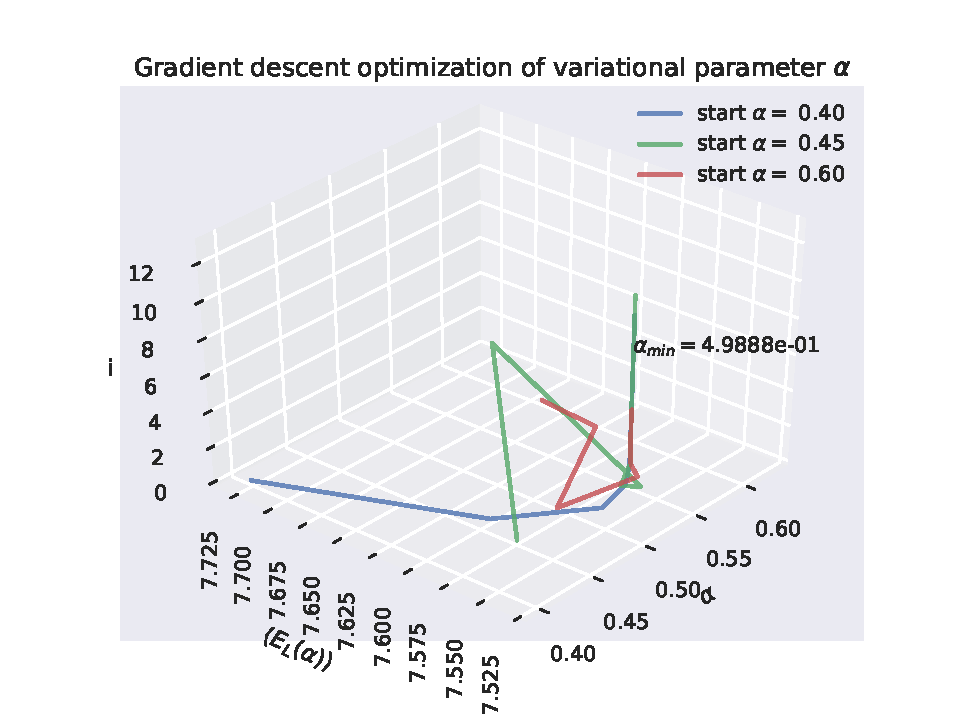
\includegraphics{figures/GD_NM_IA.pdf}
\caption{Finding the optimal $\alpha$ with GD. This plot shows the first central moment for the local energy on the y-axis, the variational parameter on the x axis and the GD iteration number on the z-axis for the interactive spherical trap. We observe that the GD algorithm finds a satisfyingly stable minimum with few iterations}\label{fig:gd_nm_ia}
\end{figure} 

\subsection*{\textbf{1g:} Onebody densities}

The onebody density was computed by counting particles in equipartitioned bins around the origo. The origo was chosen as a referemce because it is the natural focal point of particles in the harmonic oscillator trap we implemented. The bins were equipartitioned by a set step length trivially determined as $\Delta L = L/n_{bins}$ where $L$ denotes the endpoint of the interval and $n_{bins}$ the total number of bins. Each of those bins were normalized by the total count number and a factor corresponding to the difference in physical space occupied by each bin i.e. $1$ for the $1D$ case, $r$ for the $2D$ case and finally $r^2$ for the $3D$ case. The implementation of the algorithm can be found in \lstinline{vmc.cpp}. A simulation was run to compute the onebody densities for both the interactive and non-interacitve case for the respective minimas of the variational parameter $\alpha$. 

\begin{figure}
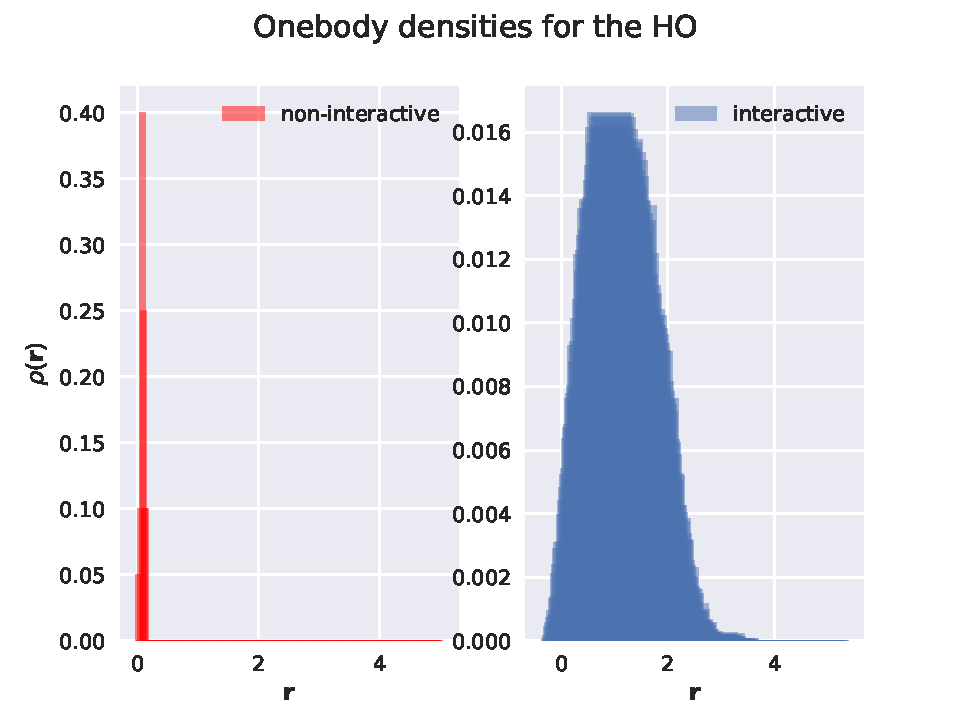
\includegraphics{figures/obd_i_ni.pdf}
\caption{With the optimal parameters for alpha the onebody densities are computed and shown above. We observe that the jastrow factor has a large and pronounced effect on the relative distribution of particles. Additionally we note that for the non-interactive case we expect a density that approximates a delta function as figuratively all bosons will be in the HO ground state.}\label{fig:obd_i_ni}
\end{figure} 